%%% Poster for ASE 2009 by Martin Weiglhofer

\documentclass[final,hyperref={pdfpagelabels=false},unknownkeysallowed]{beamer} % unknownkeysallowed to avoid errors in beamer class definitions

\mode<presentation> {  
  \usetheme{LooBa}    
}

\setbeamertemplate{caption}[numbered]

\usepackage[english]{babel}
\usepackage[utf8]{inputenc}
\usepackage{amsmath,amsthm, amssymb, latexsym}
\usepackage{epsfig}
\usepackage{multirow}
\usepackage{pifont}
\usepackage{setspace}
\usepackage{algpseudocode}
\usepackage{colortbl}
\usepackage{booktabs}
\usepackage{xcolor}
\usepackage{booktabs}

\newcommand{\Break}{\State{\textbf{break}}}

\newcommand{\no}{\color{lborange} \ding{55}}
\newcommand{\yes}{\color{lbgreen} \ding{51}}

\usepackage{tikz}
\usepackage{pgflibraryshapes}
\usetikzlibrary{arrows}
\usetikzlibrary{shapes}
\usetikzlibrary{automata}
\tikzstyle{model_node}=[circle,draw=black,fill=tuggreen!50,minimum size=50pt]
\tikzstyle{tool}=[draw,double,rounded corners,inner sep=10pt]
\tikzstyle{aut_node}=[circle,draw=black,fill=black,inner sep=0pt,minimum size=7pt,font=\footnotesize]

\usefonttheme[onlymath]{serif}
\boldmath
\usepackage[orientation=portrait,size=a0,scale=1.4,debug]{beamerposter}                       

\pgfdeclareimage[height=10cm]{institute-logo}{images/acl_wassa}
\logoleft{\pgfuseimage{institute-logo}\vspace*{-0.5cm}}

\pgfdeclareimage[height=10cm]{university-logo}{images/logo3}
\logoright{\pgfuseimage{university-logo}}

\institute[LORIA, Université de Lorraine, CNRS] 
{
  \normalsize $^1$ LORIA, Université de Lorraine, CNRS, \enspace $^2$ Université du Luxembourg
}

\date[WASSA 2024] 
{WASSA @ ACL 2024}

\subject{WASSA 2024}

\title{SentEmoContext: Context-Aware Metric Learning for Efficient Emotion Recognition in Conversation}
\author[Gendron \& Guibon]{\normalsize Barbara Gendron$^{1,2}$ and Gaël Guibon$^1$}
\mail{barbara.gendron@loria.fr}
\webpage{https://b-gendron.github.io/}

\begin{document}

\begin{frame}

\centering
\vspace{-1ex}
\begin{minipage}{0.715\textwidth}
  \begin{block}{\textbf{Motivations}}
    \begin{itemize}
      \item \enspace Information from the \textcolor{lbmagenta}{conversational context} is essential to ensure an accurate understanding of emotions in a dialog between humans.
      \item \enspace There already exist models that perform \textcolor{lbmagenta}{Emotion Recognition in Conversation} (ERC), but they often consist in intricate architectures that require high computing power.
    \end{itemize}
    \vspace{1ex} % Add space after the itemize environment
    \textbf{
      \begin{minipage}{\textwidth}
        \centering
        We propose a lightweight yet efficient model based on \textcolor{lbmagenta}{contrastive learning} to perform ERC
      \end{minipage}
      }
      \vspace{-2.5ex} % Remove the extra space at the bottom of the block
    \end{block}
  
\end{minipage}
\quad
\begin{minipage}{0.265\textwidth}
\begin{exampleblock}{\textbf{Research Questions}}
    \vspace*{2pt}
    \begin{itemize}
      \item \textbf{RQ1:} How to use the information from the conversational context to guide ERC?
    \end{itemize}
      \vspace{1ex}
    \begin{itemize}
      \item \textbf{RQ2:} Does taking into account the conversational context help to improve ERC in dyadic dialogues?
    \end{itemize}
    % \end{minipage}
    \vspace{-1ex}
\end{exampleblock}
\end{minipage}

\begin{block}{\textbf{Approach - the Training Procedure}}
 (1) builds contextual utterance representations by deploying attention, (2) specifies contextual information for emotion prediction and (3) preforms prediction on utterance triplets ($A$, $P$, $N$) where $A$ and $P$ are from the same class and $N$ is from another one.
\begin{figure}
  \centering
  \includegraphics[width=0.9\textwidth]{images/contextual_utterances_training_veryFlat.png}
  \caption{Training procedure for conversation-aware emotion predictions. Both losses (CE and triplet) backpropagate to train the encoder.}
\end{figure}
\vspace{-1ex}
\end{block}

  \begin{minipage}{0.475\textwidth}
    \begin{block}{\textbf{Experimental Setup}}
\begin{center}
  \textbf{The DailyDialog dataset \textcolor{aclblue}{\small(Li et al., 2017)}}
\end{center}
\begin{itemize}
  \item \enspace 13,118 dyadic dialogues in English about daily life concerns
  \item \enspace \textcolor{lbmagenta}{Utterance-wise} emotion annotation (\texttt{no emotion, happiness, anger, disgust, fear, surprise, sadness})
\end{itemize}
\vspace{2ex}
\begin{center}
\textbf{Metric learning with Siamese Networks \textcolor{aclblue}{\small(Koch et al., 2015)}}
\end{center}
\begin{itemize}
  \item\enspace Flexible classification framework: learns \textcolor{lbmagenta}{relations between labels}, adapts to unseen classes
  \item\enspace Intrinsic adaptation to few-shot learning to learn little-represented emotions 
  \item\enspace Weight updates using \textcolor{lbmagenta}{triplet loss} help mitigate  \textcolor{lbmagenta}{class imbalance} issue
\end{itemize}
\vspace{2ex}
\begin{figure}
  \centering
  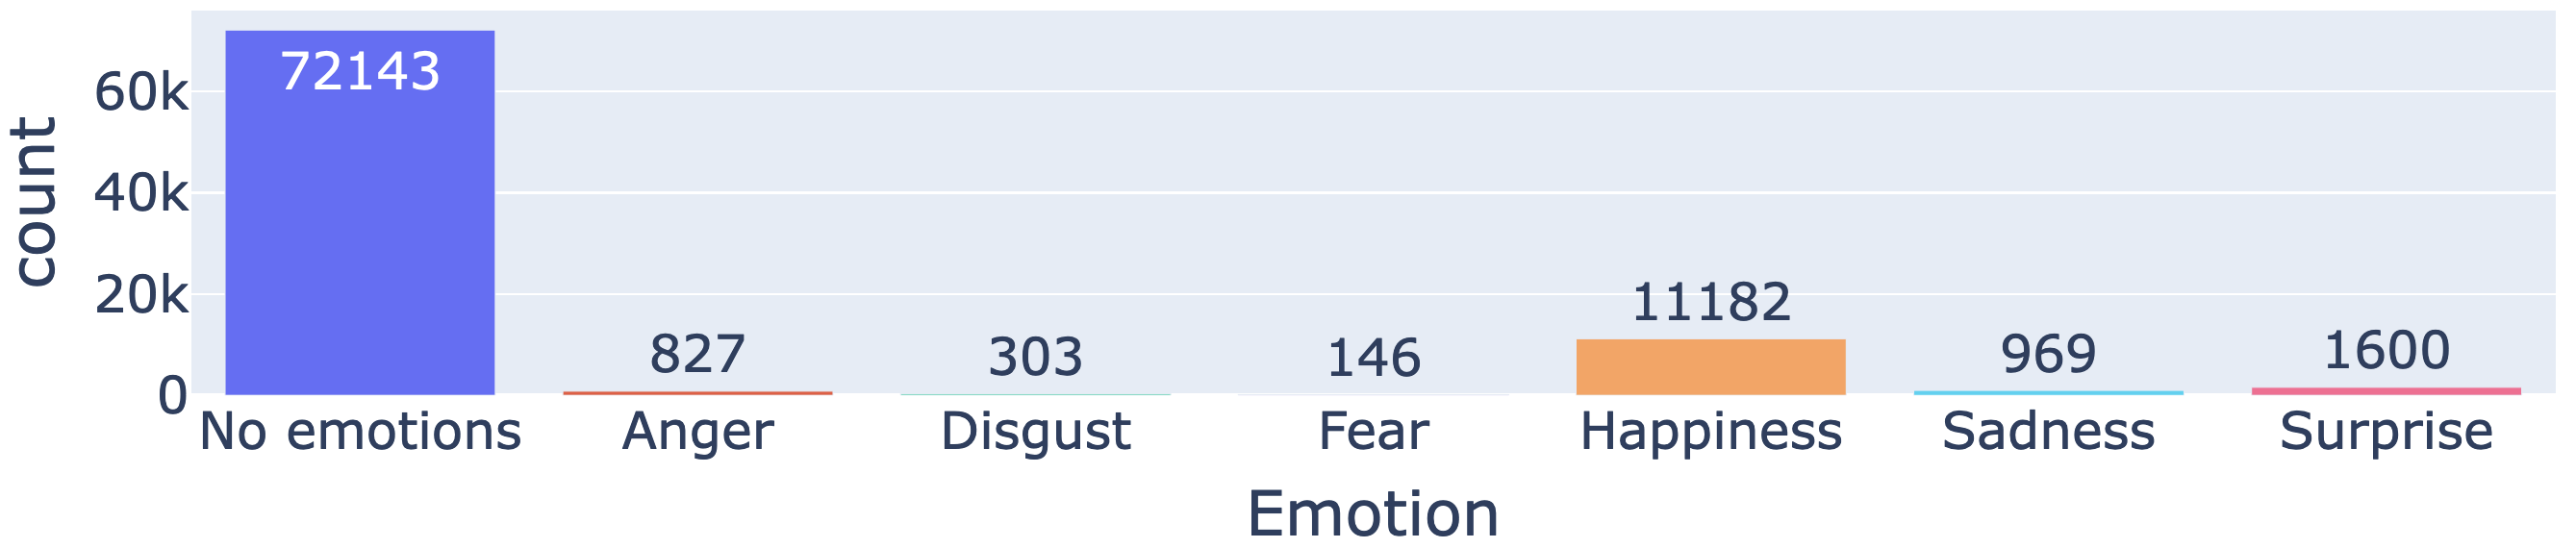
\includegraphics[width=\textwidth]{images/emo-dist-veryFlat.png}
  \caption{Label distribution in DailyDialog training set.}
\end{figure}
\vspace{1ex}
\begin{center}
  \textbf{Evaluation metrics in addition to microF1}
\end{center}
\begin{itemize}
  \item\enspace \textcolor{lbmagenta}{Macro F1}: more demanding metric that favors versatile emotion recognition
  \item\enspace \textcolor{lbmagenta}{MCC} (\textsl{Matthews Correlation Coefficient}): correlation coefficient between actual and predicted samples for a given class
\end{itemize}
\vspace{-1ex}
    \end{block}
\end{minipage}
\quad
\begin{minipage}{0.505\textwidth}
\newcommand{\mysp}{{\color{block body.bg}0}}
    \begin{block}{\textbf{Results} {\color{block title.bg}p}}
\begin{center}
    \begin{table}[!ht]
      \centering
      \begin{tabular}{@{}llll@{}}
      \toprule
      \textbf{Model name}                                        &\textbf{ macro F1*}    & \textbf{micro F1*}   &  \textbf{MCC} \\ \midrule
      \multicolumn{4}{c}{\textit{State-of-the-art models on ERC}}\\ \midrule
      CNN+cLSTM \textcolor{aclblue}{(Poria et al., 2017)}        & --                    & 50.24                & -- \\
      KET \textcolor{aclblue}{(Zhong et al., 2019)}                       & --                    & 53.37                & -- \\
      COSMIC \textcolor{aclblue}{(Ghosal et al., 2020)}                      & 51.05                 & 58.48                & -- \\
      RoBERTa \textcolor{aclblue}{(Ghosal et al., 2020)}                     & 48.20                 & 55.16                & -- \\
      Rpe-RGAT \textcolor{aclblue}{(Ishiwatari et al., 2020)}              & --                    & 54.31                & -- \\
      Glove-DRNN \textcolor{aclblue}{(Ghosal et al., 2021)}               & 41.8                  & 55.95                & -- \\
      roBERTa-DRNN \textcolor{aclblue}{(Ghosal et al., 2021)}             & 49.65                 & 57.32                & -- \\
      CNN \textcolor{aclblue}{(Ghosal et al., 2021)}                      & 36.87                 & 50.32                & -- \\
      DAG-ERC \textcolor{aclblue}{(Shen et al., 2021)}                     & --                    & 59.33                & -- \\
      TODKAT \textcolor{aclblue}{(Zhu et al., 2021)}                        &  \underline{52.56}    & 58.47                & -- \\
      SKAIG \textcolor{aclblue}{(Li et al., 2021)}                     & 51.95                 & 59.75                & -- \\
      Sentic GAT \textcolor{aclblue}{(Tu et al., 2022)}                                 & --                    & 54.45                & -- \\
      CauAIN \textcolor{aclblue}{(Zhao et al., 2022)}                                & --                    & 58.21                & -- \\
      DialogueRole \textcolor{aclblue}{(Ong et al., 2022)}                       & --                    & 60.95                & -- \\
      S+PAGE \textcolor{aclblue}{(Liang et al., 2022)}                         & --                    & \textbf{64.07}       & -- \\
      DualGAT \textcolor{aclblue}{(Zhang et al., 2023)}                    & --                    & \underline{61.84}    & -- \\
      CD-ERC \textcolor{aclblue}{(Pereira et al., 2023)}                   & 51.23                 & --                   & -- \\
      MCM-CSD \textcolor{aclblue}{(Xu and Yang, 2024)}                                   & --                    &  60.70               & --  \\
      \midrule
      \multicolumn{4}{c}{\textit{Ours}}\\ \midrule
      \texttt{SentEmoContext}                                          &  \textbf{57.71}       &  57.75            & \textbf{0.49}\\
      \bottomrule
      \end{tabular}
      \vspace{1ex}
      \caption{\centering All results for ERC on DailyDialog. * indicates metrics do not include neutral label.}
      \end{table}
  \end{center}
\vspace{-1ex}
  \end{block}
  \end{minipage}

\begin{minipage}{\textwidth}
  \begin{block}{\textbf{Comparison with Large Language Models (LLMs)}}
  \begin{minipage}{0.4\textwidth}
    \vspace{1ex}
    \begin{table}[!ht]
      \centering
      \begin{tabular}{@{}lccc@{}}
      \toprule
      \textbf{Model name}         &\textbf{ macro F1*} & \textbf{micro F1*} & \textbf{MCC} \\ \midrule
      \texttt{llama2-7b-chat-hf}  &  9.70  &  24.92     &  0.08   \\
      \texttt{llama2-13b-chat-hf} &  22.26   &   43.37  &  0.15   \\
      \texttt{falcon-7b-instruct} &  07.54   &  42.75  &  0.01 \\ 
      \midrule
      \multicolumn{4}{c}{\textit{Ours}}\\ \midrule
      \texttt{SentEmoContext}                                          &  \textbf{57.71}       &  57.75            & \textbf{0.49}\\
      \bottomrule
      \end{tabular}
      \end{table}
  \end{minipage}
  \begin{minipage}{0.55\textwidth}
      \begin{itemize}
        \item \enspace The tested LLMs performed poorly in zero-shot emotion prediction, while being far bigger that \texttt{SentEmoContext}
        \item \enspace Finding the right prompting strategy is challenging
        \item \enspace The MCC values suggest that the emotion predictions are close to random in that case: the task is not well understood in such setting
      \end{itemize}
  \end{minipage}
  \vspace{-1ex}
\end{block}
\end{minipage}


\begin{minipage}{\textwidth}
  \begin{alertblock}{\textbf{Take Home Messages}}
  \begin{minipage}{0.75\textwidth}
    \begin{itemize}
      \item \enspace We propose a novel metric-based approach to perform emotion recognition in conversation
      \item \enspace \texttt{SentEmoContext} is state-of-the-art in Macro F1, and consists in a versatile and efficient emotion prediction 
      \item \enspace Incorporating context information leads to instability issues because of noise propagation
      \end{itemize}
  \end{minipage}
  \begin{minipage}{0.23\textwidth}
    \centering
    \includegraphics[scale=0.18]{images/gh-code-big.png}
  \end{minipage}
\end{alertblock}
\end{minipage}


\end{frame}     

\end{document}


%%% Local Variables: 
%%% mode: latex
%%% TeX-master: t
%%% TeX-PDF-mode: t
%%% End: 
